\chapter{Problem Analysis}
This chapter examines existing literature concerning source localisation from EEG measurements. At first a motivation for the problem is given, considering especially the application within the hearing aid industry. Further, the state of the art methods are presented followed by a description of the contribution proposed in this thesis. 

\section{Motivation}
(Hvad er EEG)\\
EEG recordings or measurements are used within medicine as an imaging technique measuring electric signals on the scalp, caused by brain activity. \\
\\
The brain consist of an enormous amounts of cells, called neurons. These neurons are mutually connected in neural nets and when a neuron is activated, for instance by some physical stimuli, local current flows are produced\cite{fundamentalEEG}. As such the neurons are somehow communicating(?). \\
\\
The EEG measurements are provided by a varies number of metal electrodes referred to as sensors, placed on the scalp of a human reading electrical signals which are massively amplified and displayed on the computer as a sum of sinusoidal waves relative to time.\\
It takes a large amount of active neurons to generate an electrical signal that is recordable on the scalp as the current then have to penetrate the skull, skin and several other thin layers.  \\
From this it is clear that the measurements from a single sensor do not correspond to the activity of a single neuron in the brain, but rather a collection of many activities. Here the same neuron activities can be measured by two or more sensors. Furthermore, interfering signals can occur resulting from physical movement of e.g. eyes and jawbone\cite{fundamentalEEG}.\\
\\
The waves resulting from EEG have been classified into four groups according to the dominant frequency. The delta wave ($0.5-4$ Hz) is observed from infants and sleeping adults, the Theta wave ($4-8$ Hz) is observed from children and sleeping adults, the alpha wave ($8-13$ Hz) is the most extensively studied brain rhythm, which is induced by an adult laying down with closed eyes. Lastly the beta wave ($13-30$ Hz) is considered the normal brain rhythm for normal adults, associated with active thinking, active attention or solving concrete problems\cite[p. 11]{EEGsignalprocessing}. An example of EEG measurement within the four categories are illustrated 
by figure \ref{fig:EEG_example}.        
\begin{figure}[h]
    \centering
    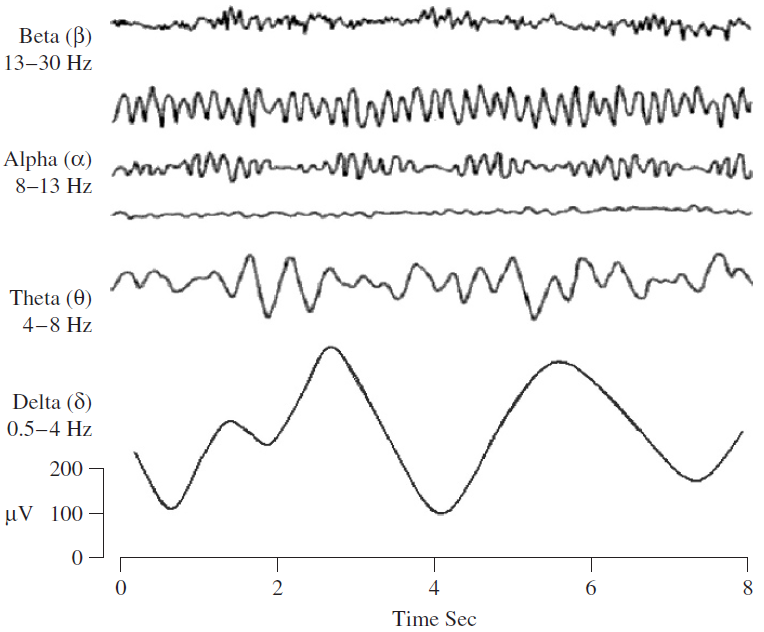
\includegraphics[scale=0.65]{figurs/EEG_example.png}
    \caption{Example of time dependent EEG measurements within the four defined categories alpha, beta, theta and delta. Image source: \cite{EEGsignalprocessing}}
    \label{fig:EEG_example}
\end{figure}

(Hvad bruges det til)\\
EEG is widely used within the medicine field and especially  research of the cognitive processes in the brain. Diagnosis and Management of neurological disorders such as epilepsy is one example. \\   

Due to EEG being non-invasive and fast it is widely used to study of the dynamical behaviour of the brain. Neural activity can be measured within fractions of a second after a stimuli has been provided\cite[p. 3]{fundamentalEEG}. When a person is exposed to certain stimuli, e.g. visual or audible, the measured activity is said to result from evoked potential.\\
Over the past two decades especially functional integration has become an area of interest, that is the interplay between functionally segregate brain areas\cite{Van2019}(evt. friston 2011). This concerns the localization of the single cortical sources causing the united signal measured by a EEG sensor.\\ 
\\

The hearing aid industry is one example where this research is highly prioritised. At Eriksholm research center which is a part of the hearing aid manufacture Oticon cognitive hearing science is a research area within in fast development. One main purpose is to make it possible for a hearing aid to identify the attended sound source by reading the signal from the brain of the user, which is where the EEG measurements are used\cite{Emina2019}\cite{Bech2018}. It is essentially the well known but unsolved cocktail problem which is sought improved by use of EEG measurement. The focus of the research considers the correlation between EEG measurements and the sound source rather than identification of the activated source from the EEG. Hence this localisation approach regarding hearing aids is of interest. Furthermore a real-time application to provide feedback from EEG measurements would be essential. \\ \\

(Modellering)\\
When considering the issue of identifying and localizing the activated sources from the EEG measurements, one known option is to model the data by the following linear system 
\begin{align*}
\mathbf{Y} = \mathbf{AX},
\end{align*}
where $\mathbf{Y} \in \mathbb{R}^M\times N_d$ is the EEG measurements from $N$ sensors at $N_d$ data points, $\mathbf{A} \in \mathbb{R}^{M \times N}$ is an unknown mixing matrix and $\mathbf{X} \in \mathbb{R}^N \times N_d$ is the actual activation of sources within the brain. The $i^{th}$ column of $A$ represent the relative projection weights from the $i^{th}$ source to every sensor or channel\cite{phd2015}. 
From this model the aim is to identify both $A$ and $X$ given the measurements $Y$. This set up is in general referred to as the inverse EEG problem.  \\
\\
To solve the problem the concept of compressive sensing makes a solid foundation including sparse signal recovery and dictionary learning. Independent Component Analysis (ICA) is a common applied method to solve the inverse problem\cite{Scott1996}\cite{Scott1997}, here statistical independence between source activity is assumed. \\
Application of ICA have shown great results regarding separation of high-density EEG. Further an enhanced signal-to-noise ratio of the unmixed independent source time series processes allow essential study of the behaviour and relationships between multiple EEG source processes\cite{Arnaud2012}. However a significant flaw to this method is that to the EEG data can only be separated into a number of sources that are equal or less than the number of sensors, that is the inverse EEG problem can not be over-complete. This assumption undermines the reliability and usability of ICA, as the number of simultaneous active sources easyly  exceed the number of sensors\cite{phd2015}. This is especially a drawback when low density EEG are considered, that is equipment with less than 32 sensors. However improved capabilities of low density EEG devices are desirable due to relative low cost, mobility and ease to use. \\  
\\
This makes a foundation to look at the existing work considering the overcomplete inverse EEG problem. 

\section{Related Work and Our Contribution} 
As mentioned above ICA have been a solid method for source localisation in the case where a decomposition into a number of sources equal to the number of sensors was accepted. To overcome this issue an extension of ICA was suggested, referred to as the ICA mixture model, insted of identifying one mixing matrix $\mathbf{A}\in \mathbb{R}^{M\times N}$ this approach learns $N_{model}$(number of sources?) different mixing matrices $\mathbf{A}_i\in \mathbb{R}^{M\times M}$. A further adaptation of this method AMICA(Adaptive Mixture ICA) have shown successful results regarding identification of more sources than available sensors\cite{Palmer2008}. However an assumption of no more than $M$ simultaneously active sources has to be made which is still an essential limitation, especially when considering low density EEG. \\
Other types of overcomplte ICA algorithms have been proposed to overcome the problem of learning overcomplete systems. One is the Restricted ICA, an efficient method used for unsupervised learning in neural networks\cite{Le2011}. Here the hard orthonormal constraint in ICA is replaced with a soft reconstruction cost.\\
In 2015 O. Balkan suggested a new approach also targeting the identification of more sources than sensors regarding EEG \cite{Balkan2015}. The suggested method referred to as Cov-DL is a covariance based dictionary learning algorithm. The point is to transfer the forward problem into the covariance domain which has higher dimensionality than the original EEG sensor domain. This can be done when assuming the scalp mixing is linear   using the assumed natural uncorrelation of sources within a certain time-window. The Cov-DL algorithm stands out from the other straight forward dictionary learning methods as it does not relay on the sparsity of active sources thus it is a further advantage when low density EEG is considered. \\
Cov-DL was found to outperform both AMICA and RICA, thus it is considered the state of the art within the area of source identification. \\ \\
It is essential to note that the Cov-DL algorithm do only learn the mixing matrix $A$, the projection of sources to the scalp sensors, and not the explicit source activity time series $X$.\\
For this purpose a multiple measurement sparse
bayesian learning (M-SBL) algorithm was proposed in 2014 also by O. Balkan, targeting the case of more active sources than sensors\cite{Balkan2014}. Here the mixing matrix which is now assumed known should fulfil the exact support recovery conditions. Though the method was proven to outperform the recently used algorithm M-CoSaMP even then the defined conditions was not fulfilled.  \\   
\\
The two state of the art methods for source identification will make the foundation of this thesis. This project propose an algorithm which uses the investigated methods on synthetic EEG data and real EEG data.
Further, the purpose is to extend the algorithm to perform on EEG measurement in real-time in order to investigate the possibility of providing useful feedback depending on the real-time results of the algorithm. 
For this analysis of results in different sound environments such as noisy and noise-less cases and cases of directional noise.\\
The overall purpose of the real-time performance is to provide results that can be useful to the hearing aid industry, considering the development of self-adaptive hearing aids.
By this extension and associated analysis we seek to extend the existing results within the area.   
\\ \\


nb. husk at dette kapitel skal vise et helt system og hvorhenne i det system vi kigger nærmere og kommer ind med vores bidrag. Det skal gøres klar hvilke områder vi vælger at ligge vores kræfter i.  





 
